\documentclass[10pt,a4paper]{article}
\usepackage[T1]{fontenc}
\usepackage[utf8]{inputenc}
\usepackage{lmodern,microtype}
\usepackage[margin=.8in]{geometry}
\usepackage{amsmath,amssymb,amsthm,booktabs,tabularx,array,enumitem,mdframed}
\usepackage{xcolor}
\usepackage{tikz}
\usetikzlibrary{arrows.meta,calc}
\definecolor{rrBlue}{HTML}{2563EB}
\definecolor{rrTeal}{HTML}{0F766E}
\definecolor{rrAmber}{HTML}{B45309}
\definecolor{rrRed}{HTML}{B91C1C}
\definecolor{rrGray}{HTML}{475569}
\tikzset{
 rrflow/.style={-{Stealth[length=2mm]},line width=.85pt,draw=rrGray},
 rrdot/.style={circle,inner sep=0pt,minimum size=4pt,fill=rrTeal},
 rrnote/.style={align=center,font=\sffamily\footnotesize,inner sep=2pt},
 rrbox/.style={draw=rrGray!60,rounded corners=3pt,fill=white,
  align=center,font=\sffamily\small,inner sep=6pt},
 rraxis/.style={-{Stealth[length=1.5mm]},draw=rrGray!70,line width=.5pt}}
\newcommand{\pipelinecaption}[2]{\refstepcounter{figure}\label{#1}\par\smallskip
 {\small\textbf{Figure~\thefigure.} #2\par}\medskip}
\usepackage[hidelinks]{hyperref}
\hypersetup{pdftitle={Regular Rotation in Sync HotStuff -- V5},pdfsubject={Agreed recovery with the original fast-path timer}}
\setlength{\parindent}{0pt}
\setlength{\parskip}{4pt}
\setlength{\emergencystretch}{2em}
\setlist{nosep,leftmargin=*}
\newcolumntype{Y}{>{\raggedright\arraybackslash}X}
\newcommand{\QC}{\mathsf{QC}}
\newcommand{\BC}{\mathsf{BC}}
\newcommand{\IC}{\mathsf{IC}}
\newcommand{\chg}[1]{\textcolor{red!70!black}{#1}}
\newtheorem{lemma}{Lemma}
\newtheorem{theorem}{Theorem}
\begin{document}
\begin{center}
{\Large\bfseries Regular Rotation in Sync HotStuff: V5}\\[3pt]
{\large Original fast-path timer; agreed recovery on failure}\\[3pt]
11 October 2026
\end{center}

\textbf{Scope.} V5 makes equivocation detection and its immediate effect
explicit in the two protocol boxes. It preserves V4's regular rotation,
vote-start $2\Delta$ timer, common failure recovery, and proofs.
This is a count-based SMR reference, not an implementation of the weighted
regional service in \texttt{main\_v3.tex}. V1--V4 remain separate files.

\textbf{Model.} Fixed membership, $n=2f+1$, at most $f$ Byzantine replicas,
unforgeable signatures, equal-rate clocks, and known correct-to-correct
complete-message delay $\Delta$, including validation. At exact boundaries,
process received messages before timers. Empty batches are available.

\textbf{One view identity, one leader.} A view is $V=(e,r)$, ordered
lexicographically. Epoch $e$ changes only after failure recovery; normal
rotation increments $r$. The leader is the deterministic function
$L(e,r)=L_{r\bmod n}$ of this view identity, not a separately elected variable.
Every signed message binds its type, epoch, term, height and block/context
hashes. Voting identities are never reused across epochs.
Epoch $e$ starts with a common committed base $A_e$, height $H_e$, and term
$r_e$. Term $r\ge r_e$ owns fresh positions
\[
 H_e+(r-r_e)K+1,\ldots,H_e+(r-r_e+1)K,\qquad K\ge1.
\]
A normal entry requires the complete chain of intervening terminal QCs.
A QC contains $f+1$ matching votes. Rank it lexicographically by
$(e,r,h(B),\mathsf{H}(B))$; the hash supplies a deterministic tie-break.
The agreed base is the fallback below all fresh current-epoch QCs.
A quit proof is either $f+1$ BLAME signatures for one admissible $(e,r)$
or two distinct, correctly attributed leader-signed PROPOSE objects at the
same $(e,r,h)$ with different block digests and verifiable full ancestry.
The latter is a leader-equivocation witness; one BLAME share or a second
signature on the same digest is not. Initial entries share $A_0,r_0$ and
differ in time by at most $\Delta$.

\begin{mdframed}[linewidth=.6pt,innertopmargin=5pt,innerbottommargin=5pt]
\textbf{Protocol 1. Steady state (original Figure 1 structure).}
\begin{enumerate}[label=\textbf{\arabic*.},itemsep=3pt]
\item \textbf{Propose.} An unfrozen correct leader immediately broadcasts the next
valid fresh child when its certified parent is available and its quota
has an unused slot (including immediately on entry). \chg{The first child of a normal term may use the preceding
terminal QC; the first term of an epoch may extend its agreed base $A_e$.}
\item \textbf{Echo, equivocation check, and vote.} On \emph{every}
authenticated PROPOSE or QC bundle for the current epoch, inspect its
complete signed ancestry against retained histories, including earlier
normal terms. \chg{At the first incompatible slot, broadcast the two
original leader-signed PROPOSE objects and their verification paths;
immediately invoke Protocol 2(i), without waiting for BLAME signatures.
Do not vote on either newly received conflicting branch.}
If the history is compatible and already past $B$, relay $\QC(B)$ without
re-voting. Otherwise, while unfrozen, catch up through terminal QCs;
if $B$ is eligible in the resulting active term and this slot has not
been voted, relay the signed proposal, multicast a vote and start its
$2\Delta$ commit timer. Never double-vote at $(e,r,h)$. Assemble and relay
QCs independently of the leader. \chg{A terminal QC advances to $(e,r+1)$
immediately, disarms that term's missing-progress listener, and preserves
its pending commit timers.}
\item \textbf{Commit (non-blocking).} At timer expiry, process all
received proof messages first. Commit the block and ancestors only if the
epoch is not frozen and no admissible leader equivocation is known.
\chg{Protocol 2 cancels all outstanding epoch timers on a quit proof.}
No QC-at-expiry guard is added. Never revoke a commit; reject votes
conflicting with the committed prefix.
\end{enumerate}
\end{mdframed}

\begin{mdframed}[linewidth=.6pt,innertopmargin=5pt,innerbottommargin=5pt]
\textbf{Protocol 2. View change (original Figure 2 structure).}
\begin{enumerate}[label=\textbf{\roman*.},itemsep=3pt]
\item \textbf{Blame, evidence, and quit.} At
$s_i(e,r)+(2p+4)\Delta$, send signed BLAME$(e,r)$ if fewer than $p$
valid fresh proposals are known, for $1\le p\le K$, and no complaint
is pending; mark this complaint pending. On $f+1$ matching
signatures, assemble the complete $\BC_{(e,r)}$; a lone signature never
quits. \chg{On that certificate or a verified pair of conflicting
leader-signed PROPOSE messages, immediately broadcast the complete witness,
freeze the entire current epoch at $a_i$, stop new votes/normal entry, and
cancel every outstanding epoch commit timer, including timers from earlier
normal terms.} Keep completed commits. During the $\Delta$ wait, continue
relaying old proposals and votes and assembling QCs; collect later proofs
without restarting recovery.
\item \textbf{Status.} Wait $\Delta$. \chg{Snapshot all known current-epoch
QCs and quit proofs, including complete admission ancestry. Use the
failure-only agreement in the \hyperref[sec:agreement]{recovery specification} to obtain a common
vector containing every correct snapshot.}
\item \textbf{New-view.} \chg{From that common vector select the smallest
admissible blamed term $b$ and the highest admissible current-epoch QC
(or $A_e$ if none). Let its block be $A_{e+1}$. Commit this common anchor,
and decide $V'=(e+1,b+1)$, whose leader is $L(V')$.}
\item \textbf{First vote.} \chg{Install $A_{e+1}$ and $r_{e+1}=b+1$, unfreeze,
set the new local entry clock, and resume Protocol 1. A correct new leader
immediately proposes its first fresh child. The agreed anchor needs no re-certification vote.
Retain prior records, but old-epoch proofs cannot restart this recovery.}
\end{enumerate}
\end{mdframed}


\clearpage
\section*{Illustrated normal operation}
The blue/teal stages carry proposals, votes and QCs; amber bars are local
commit timers. The first plot uses an illustrative actual one-hop delay
$\delta=\Delta/4$. This is an example execution, not an additional timing
assumption or a mandatory wait. A certified parent is already available.

\begin{center}
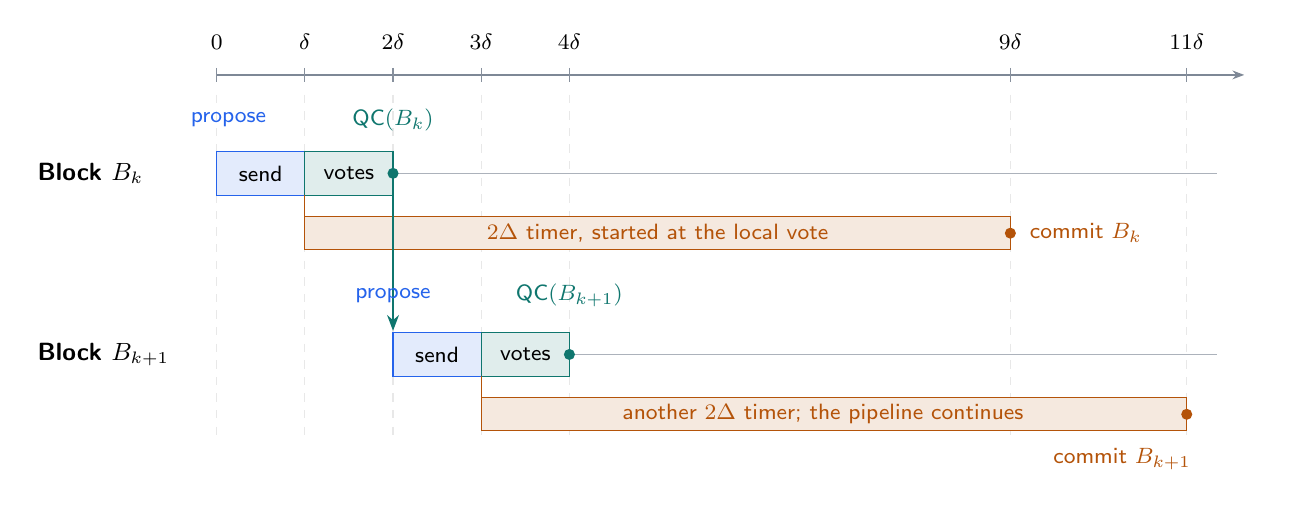
\begin{tikzpicture}[x=1cm,y=-1cm,font=\sffamily\footnotesize]
\path[use as bounding box] (0,-.15) rectangle (16,5.8);
\draw[rraxis] (2.4,.45) -- (15.45,.45);
\foreach \x/\lab in {2.4/0,3.52/\delta,4.64/2\delta,5.76/3\delta,6.88/4\delta,12.48/9\delta,14.72/11\delta}{
 \draw[rrGray!65] (\x,.36)--(\x,.54);
 \node[rrnote,anchor=south] at (\x,.2) {$\lab$};
}
\foreach \x in {2.4,3.52,4.64,5.76,6.88,12.48,14.72}
 \draw[gray!18,dashed] (\x,.7)--(\x,5.05);
\node[rrnote,anchor=west,font=\sffamily\bfseries\small] at (.05,1.7) {Block $B_k$};
\node[rrnote,anchor=west,font=\sffamily\bfseries\small] at (.05,4.0) {Block $B_{k+1}$};
\draw[rrGray!45] (2.4,1.7)--(15.1,1.7);
\draw[rrGray!45] (4.64,4.0)--(15.1,4.0);
\filldraw[fill=rrBlue!13,draw=rrBlue] (2.4,1.42) rectangle (3.52,1.98);
\filldraw[fill=rrTeal!13,draw=rrTeal] (3.52,1.42) rectangle (4.64,1.98);
\node[rrnote] at (2.96,1.7) {send};
\node[rrnote] at (4.08,1.7) {votes};
\node[rrnote,text=rrBlue] at (2.55,1.02) {propose};
\node[rrdot] at (4.64,1.7) {};
\node[rrnote,text=rrTeal] at (4.64,1.02) {$\QC(B_k)$};
\filldraw[fill=rrAmber!13,draw=rrAmber] (3.52,2.25) rectangle (12.48,2.67);
\draw[rrAmber] (3.52,1.98)--(3.52,2.25);
\node[rrnote,text=rrAmber] at (8.0,2.46) {$2\Delta$ timer, started at the local vote};
\node[rrdot,fill=rrAmber] at (12.48,2.46) {};
\node[rrnote,anchor=west,text=rrAmber] at (12.65,2.46) {commit $B_k$};
\draw[rrflow,draw=rrTeal] (4.64,1.98)--(4.64,3.7);
\filldraw[fill=rrBlue!13,draw=rrBlue] (4.64,3.72) rectangle (5.76,4.28);
\filldraw[fill=rrTeal!13,draw=rrTeal] (5.76,3.72) rectangle (6.88,4.28);
\node[rrnote] at (5.20,4.0) {send};
\node[rrnote] at (6.32,4.0) {votes};
\node[rrnote,text=rrBlue] at (4.64,3.25) {propose};
\node[rrdot] at (6.88,4.0) {};
\node[rrnote,text=rrTeal] at (6.88,3.25) {$\QC(B_{k+1})$};
\filldraw[fill=rrAmber!13,draw=rrAmber] (5.76,4.55) rectangle (14.72,4.97);
\draw[rrAmber] (5.76,4.28)--(5.76,4.55);
\node[rrnote,text=rrAmber] at (10.1,4.76) {another $2\Delta$ timer; the pipeline continues};
\node[rrdot,fill=rrAmber] at (14.72,4.76) {};
\node[rrnote,text=rrAmber,anchor=north] at (13.9,5.12) {commit $B_{k+1}$};
\end{tikzpicture}
\end{center}
\pipelinecaption{fig:normal-pipeline}{Normal proposals inside one term.
A representative nonleader receives $B_k$ at $\delta$, forwards and votes,
and starts its timer. All-to-all votes supply the QC at $2\delta$, enabling
the next proposal. Its local commit is only at $\delta+2\Delta=9\delta$,
provided no recovery cancels the timer. A QC is visibly earlier than commit.
The same pipeline is present in vanilla Sync HotStuff; QC formation does not
require the leader to collect and redistribute all votes.}

\medskip
\textbf{Regular rotation changes the producer at the QC boundary.}
Let $X$ be Alice's $K$th fresh batch and $Y$ Bob's first fresh batch. The
following is causal flow, with schematic horizontal spacing.
\begin{center}
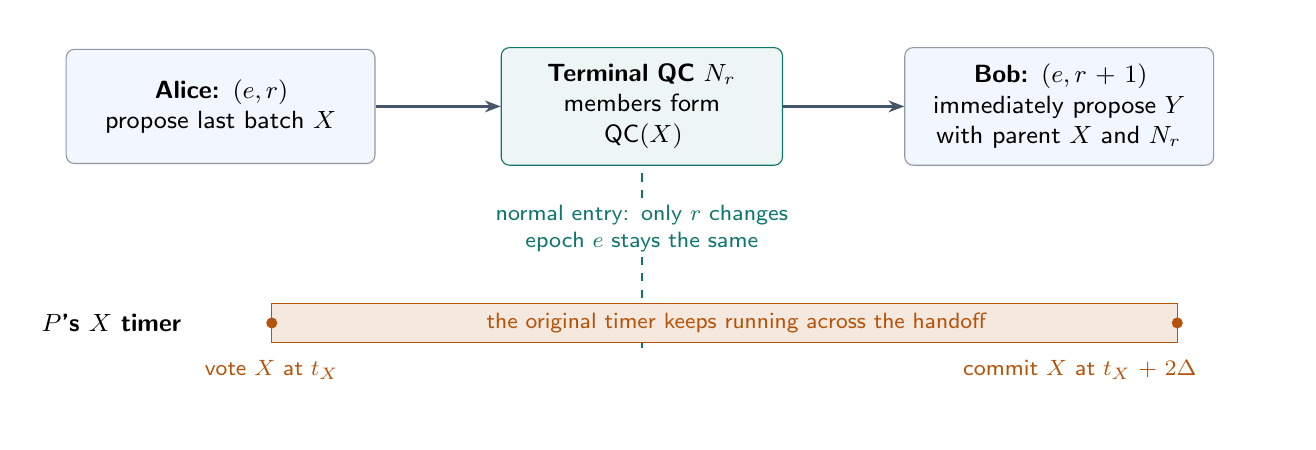
\begin{tikzpicture}[x=1cm,y=-1cm]
\path[use as bounding box] (0,0) rectangle (16,5.0);
\node[rrbox,fill=rrBlue!6,text width=3.5cm,minimum height=1.45cm] (alice) at (2.45,1)
 {\textbf{Alice: $(e,r)$}\\propose last batch $X$};
\node[rrbox,draw=rrTeal,fill=rrTeal!7,text width=3.15cm,minimum height=1.45cm] (qc) at (7.8,1)
 {\textbf{Terminal QC $N_r$}\\members form\\$\QC(X)$};
\node[rrbox,fill=rrBlue!6,text width=3.5cm,minimum height=1.45cm] (bob) at (13.1,1)
 {\textbf{Bob: $(e,r+1)$}\\immediately propose $Y$\\with parent $X$ and $N_r$};
\draw[rrflow] (alice)--(qc);
\draw[rrflow] (qc)--(bob);
\draw[rrTeal,dashed,line width=.8pt] (7.8,1.85)--(7.8,4.1);
\node[rrnote,text=rrTeal,fill=white,text width=4.1cm] at (7.8,2.55)
 {normal entry: only $r$ changes\\epoch $e$ stays the same};
\node[rrnote,anchor=west,font=\sffamily\bfseries\small] at (.1,3.75) {$P$'s $X$ timer};
\filldraw[fill=rrAmber!13,draw=rrAmber] (3.1,3.50) rectangle (14.6,4.0);
\node[rrnote,text=rrAmber] at (9.0,3.75) {the original timer keeps running across the handoff};
\node[rrdot,fill=rrAmber] at (3.1,3.75) {};
\node[rrdot,fill=rrAmber] at (14.6,3.75) {};
\node[rrnote,text=rrAmber,anchor=north] at (3.1,4.15) {vote $X$ at $t_X$};
\node[rrnote,text=rrAmber,anchor=north,text width=4cm] at (13.35,4.15)
 {commit $X$ at $t_X+2\Delta$};
\end{tikzpicture}
\end{center}
\pipelinecaption{fig:normal-rotation}{QC-driven normal handoff.
In the execution of Figure~\ref{fig:normal-pipeline}, Alice sends $X$ at 0,
Bob sends $Y$ at $2\delta$, and a follower votes for $Y$ at $3\delta$;
Alice's $X$ is still awaiting its timer. No BLAME, STATUS exchange or failure
agreement is invoked by this handoff. Full terminal-QC ancestry lets a slower
replica catch up. Only a subsequent valid quit proof cancels pending epoch
timers; already completed commits remain intact.}

\clearpage
\section*{Conflicting BLAME evidence and common recovery}
Use $n=5$, $f=2$, with Alice at term 0 and Bob at term 1. A valid old honest
BLAME share for Alice already exists. At time 0, $P$ receives $\BC_{(e,1)}$
and freezes; Caro receives it at $\Delta$. Byzantine members complete the
withheld $\BC_{(e,0)}$ at Caro at $3\Delta/2$; its relay reaches $P$ at
$5\Delta/2$. Thus the two honest STATUS snapshots differ. A single BLAME
share would not freeze either node.

\begin{center}
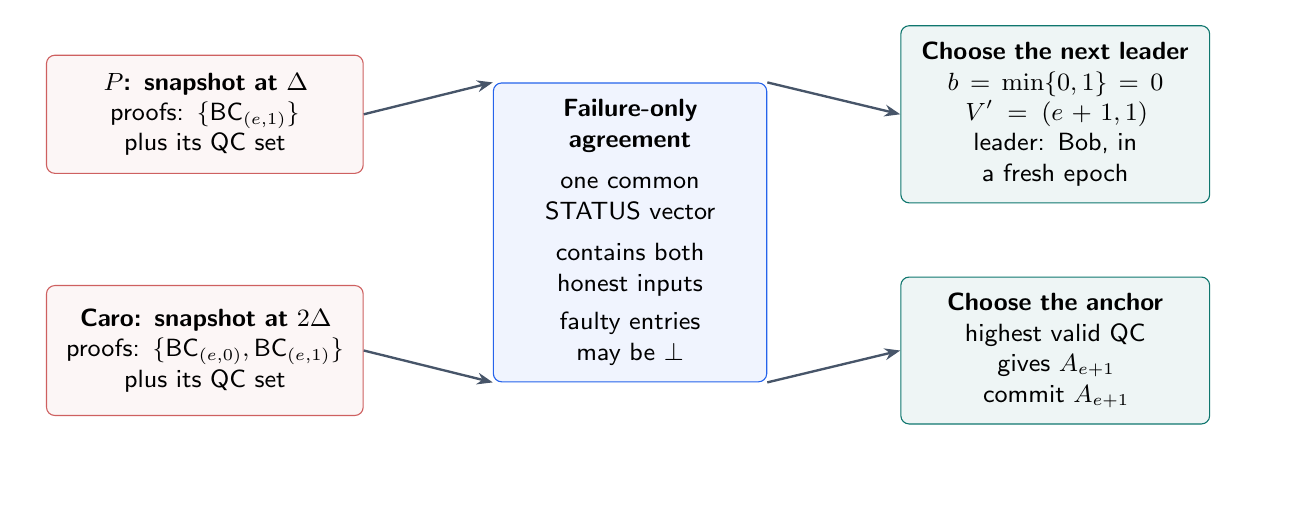
\begin{tikzpicture}[x=1cm,y=-1cm]
\path[use as bounding box] (0,0) rectangle (16,5.8);
\node[rrbox,draw=rrRed!70,fill=rrRed!4,text width=3.6cm,minimum height=1.5cm] (pstatus) at (2.25,1.1)
 {\textbf{$P$: snapshot at $\Delta$}\\proofs: $\{\BC_{(e,1)}\}$\\plus its QC set};
\node[rrbox,draw=rrRed!70,fill=rrRed!4,text width=3.6cm,minimum height=1.65cm] (cstatus) at (2.25,4.1)
 {\textbf{Caro: snapshot at $2\Delta$}\\proofs: $\{\BC_{(e,0)},\BC_{(e,1)}\}$\\plus its QC set};
\node[rrbox,draw=rrBlue,fill=rrBlue!7,text width=3.05cm,minimum height=2.8cm] (common) at (7.65,2.6)
 {\textbf{Failure-only agreement}\\[4pt]one common STATUS vector\\[4pt]contains both honest inputs\\[3pt]faulty entries may be $\bot$};
\node[rrbox,draw=rrTeal,fill=rrTeal!7,text width=3.5cm,minimum height=1.75cm] (leader) at (13.05,1.1)
 {\textbf{Choose the next leader}\\$b=\min\{0,1\}=0$\\$V'=(e+1,1)$\\leader: Bob, in a fresh epoch};
\node[rrbox,draw=rrTeal,fill=rrTeal!7,text width=3.5cm,minimum height=1.75cm] (anchor) at (13.05,4.1)
 {\textbf{Choose the anchor}\\highest valid QC\\gives $A_{e+1}$\\commit $A_{e+1}$};
\draw[rrflow] (pstatus.east)--(common.north west);
\draw[rrflow] (cstatus.east)--(common.south west);
\draw[rrflow] (common.north east)--(leader.west);
\draw[rrflow] (common.south east)--(anchor.west);
\end{tikzpicture}
\end{center}
\pipelinecaption{fig:blame-conflict}{Different inputs, identical recovery outputs.
The minimum BLAME term selects the successor; independently, the highest
admissible QC selects the anchor. ``Minimum'' refers to the common agreed
reports, not the first certificate received or every certificate ever formed.
Choosing Bob does not make him honest: $(e+1,1)$ is a fresh voting identity.
Old $\BC_{(e,1)}$ cannot abort it; a fresh failure can lead to the next recovery.}

\textbf{The recovery decision agrees in value, not necessarily in time.}
Time below is measured from the first correct freeze, in units of $\Delta$.
The earliest and latest correct starts illustrate the maximum allowed skew.
\begin{center}
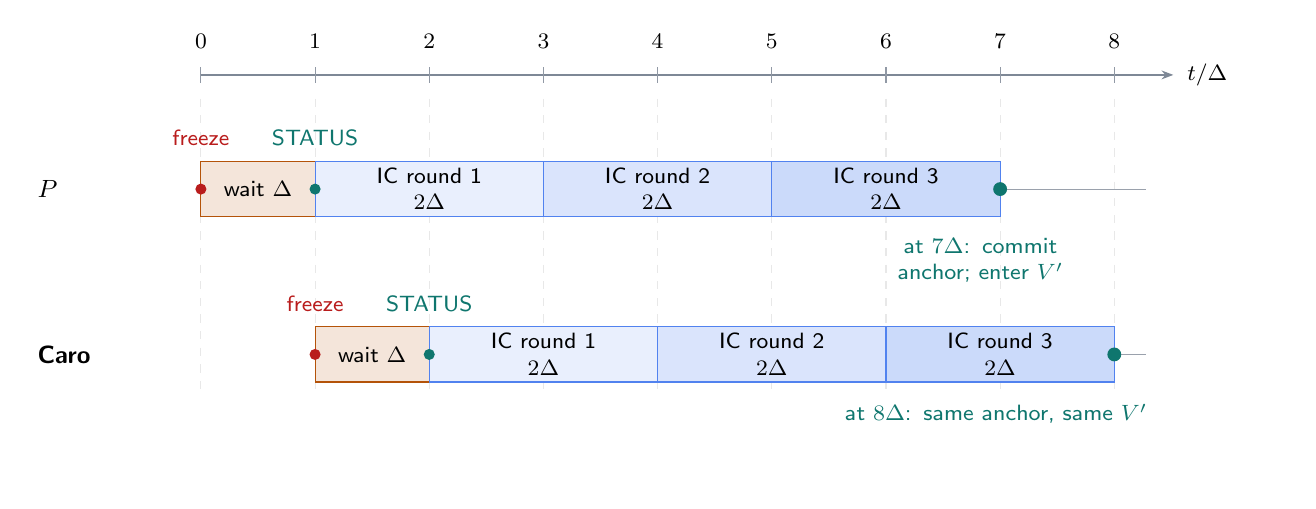
\begin{tikzpicture}[x=1cm,y=-1cm,font=\sffamily\footnotesize]
\path[use as bounding box] (0,-.15) rectangle (16,5.6);
\draw[rraxis] (2.2,.45)--(14.55,.45);
\foreach \k in {0,...,8}{
 \pgfmathsetmacro{\xx}{2.2+1.45*\k}
 \draw[rrGray!60] (\xx,.35)--(\xx,.55);
 \node[rrnote,anchor=south] at (\xx,.19) {$\k$};
 \draw[gray!18,dashed] (\xx,.75)--(\xx,4.5);
}
\node[rrnote,anchor=west] at (14.65,.45) {$t/\Delta$};
\node[rrnote,anchor=west,font=\sffamily\bfseries\small] at (.05,1.9) {$P$};
\node[rrnote,anchor=west,font=\sffamily\bfseries\small] at (.05,4.0) {Caro};
\foreach \y/\shift in {1.9/0,4.0/1}{
 \pgfmathsetmacro{\start}{2.2+1.45*\shift}
 \pgfmathsetmacro{\snap}{\start+1.45}
 \draw[rrGray!55] (\start,\y)--(14.2,\y);
 \filldraw[fill=rrAmber!15,draw=rrAmber] (\start,\y-.35) rectangle (\snap,\y+.35);
 \node[rrnote] at ({(\start+\snap)/2},\y) {wait $\Delta$};
 \node[rrdot,fill=rrRed] at (\start,\y) {};
 \node[rrnote,text=rrRed,anchor=south] at (\start,\y-.47) {freeze};
 \foreach \k/\shade in {1/10,2/17,3/24}{
  \pgfmathsetmacro{\leftx}{\snap+2.9*(\k-1)}
  \pgfmathsetmacro{\rightx}{\leftx+2.9}
  \filldraw[fill=rrBlue!\shade,draw=rrBlue!80] (\leftx,\y-.35) rectangle (\rightx,\y+.35);
  \node[rrnote] at ({(\leftx+\rightx)/2},\y) {IC round \k\\$2\Delta$};
 }
 \node[rrdot] at (\snap,\y) {};
 \node[rrnote,text=rrTeal,anchor=south] at (\snap,\y-.47) {STATUS};
}
\node[rrdot,minimum size=5pt] at (12.35,1.9) {};
\node[rrdot,minimum size=5pt] at (13.8,4.0) {};
\node[rrnote,text=rrTeal,text width=4cm,anchor=north] at (12.1,2.45)
 {at $7\Delta$: commit anchor; enter $V'$};
\node[rrnote,text=rrTeal,text width=4cm,anchor=north] at (12.3,4.55)
 {at $8\Delta$: same anchor, same $V'$};
\end{tikzpicture}
\end{center}
\pipelinecaption{fig:recovery-timing}{Failure recovery for $f=2$.
Each row runs five sender-broadcast instances \emph{in parallel}, each with
three padded rounds. The two outputs are the same despite the one-delay
start skew. A replica still finishing recovery buffers early next-epoch
messages. In general, all decisions occur by $(2f+4)\Delta$ after the first
freeze. There is no extra leader wait or anchor re-certification after this
agreement. Frozen replicas keep processing old votes and forming QCs.}

\clearpage
\section*{Equivocation and regional-model audit}
\textbf{Detection in V5.} The leader's signed PROPOSE messages bind
$(e,r,h)$ and the block digest. Two incompatible admissible histories in one
epoch first diverge at one canonical slot, whose scheduled leader must have
signed two different proposals. The observer forwards the two original
signed objects plus the missing ancestry. Any correct recipient verifies them
and freezes the epoch immediately, regardless of which normal term it is
currently serving. The observer does not wait for $f+1$ BLAME signatures.
One invalid proposal is rejected; Byzantine double-voting by a nonleader is
accountability evidence, not automatically a leader-equivocation quit proof.

\textbf{Why the NEWVIEW case differs.} In \texttt{main\_v3.tex}, the
recovering leader signs NEWVIEW and announces one anchor. Two signed NEWVIEW
messages choosing different anchors are equivocation evidence, even if those
anchors are comparable. V5's recovery agreement gives every correct party
the same anchor directly; its leader neither selects nor signs a NEWVIEW
anchor announcement. A spurious NEWVIEW message is therefore invalid in
V5, and the two-NEWVIEW trigger from the older protocol has no live message
type to compare. Failure of the new leader to propose is handled by the
missing-progress BLAME timer. These are substantive recovery changes.

\textbf{Regional integration boundary.} The V5 quorum is $f+1$ of
$2f+1$ equal-count members; \texttt{main\_v3.tex} instead assumes faulty
stake $<W_i/3$, vote QC weight $>2W_i/3$, and BLAME weight $>W_i/3$.
That manuscript additionally validates application and mini-block ranges,
producer authority and L1 references, produces post-commit CONFIRM receipts,
uses a DRAIN/quota adapter, and has a separate L1 double-head/slashing
procedure. V5's abstract
application-validity check, signed fork witness and SMR safety proof do not
instantiate those service or weighted-security rules. A regional adoption
would need those checks, thresholds and proof obligations restored explicitly.

\section*{Comparison with vanilla Sync HotStuff}
The baseline here is the standard-synchronous protocol in Figures 1--2 of
Sync HotStuff~\cite{sync}, with $n=2f+1$ and $f+1$-vote QCs. Both protocols
forward proposals, multicast votes, and start the nonblocking $2\Delta$
commit timer at the local vote. The following differences concern leader
rotation and failure recovery; the diagrams do not change the V5 rules.

\begin{center}\small
\begin{tabularx}{\linewidth}{@{}>{\raggedright\arraybackslash}p{.18\linewidth}>{\raggedright\arraybackslash}p{.32\linewidth}Y@{}}
\toprule
Aspect & Vanilla standard synchrony & V5\\\midrule
Normal leader tenure & A leader continues until failure-driven replacement. &
After $K$ fresh batches, the terminal QC enables the next scheduled leader.\\
View identity & One view index $v$. & One composite view $(e,r)$;
normal rotation increments $r$, recovery increments $e$.\\
QC versus commit & QC enables a child; the local timer supplies commit. &
Same timing; a terminal QC additionally enables a different producer
(Figures~\ref{fig:normal-pipeline}--\ref{fig:normal-rotation}).\\
First child after normal rotation & No terminal-quota handoff in the baseline. &
May use the preceding term's terminal QC as its parent certificate.\\
Progress accounting & Missing proposals are counted by triggered votes. &
Known valid proposals include certified catch-up; terminal QC disables the
completed term's missing-progress listener.\\
Quit scope & Quit the current view and cancel its timers. & Freeze the entire
current epoch and cancel all its unfinished timers; completed commits remain.\\
Equivocation & Relay two signed conflicting PROPOSE/NEWVIEW messages;
two different NEWVIEW anchors also count. & Compare complete same-epoch
proposal histories, relay the first signed same-slot fork and freeze;
there is no leader-selected NEWVIEW anchor.\\
Recovery decision & After the exit wait, report a lock; the next leader
collects statuses and chooses an anchor. & Agree on a common report vector;
minimum BLAME selects the term, highest valid QC selects the anchor.\\
Recovery anchor & Re-certify the chosen anchor without a commit timer. &
Commit the agreed safe anchor at the recovery decision; no re-certification round.\\
Recovery waits & Exit wait $\Delta$, leader wait $2\Delta$, then message
exchanges. & Snapshot wait $\Delta$, then $f+1$ authenticated-broadcast rounds
of $2\Delta$; sender instances run in parallel.\\
Old messages & Native view progression and entry locks constrain reuse. &
New epoch separates signing identities; an old-epoch quit proof cannot
restart completed recovery.\\\bottomrule
\end{tabularx}\end{center}

\textbf{What normal rotation saves.} The producer changes at the same QC
boundary that already enables the next block. In Figure~\ref{fig:normal-rotation},
Bob does not wait for Alice's final timer. No failure-agreement round is
paid for a successful handoff. The normal proposal interval and local
vote-start timer remain those illustrated in Figure~\ref{fig:normal-pipeline}.
This does not make a QC a finality certificate by itself.

\textbf{Why failure recovery changes more.} Normal advancement can put
replicas in different terms when delayed BLAME certificates appear.
Independent local minima need not match. V5 first closes a common evidence
set, then derives both the next view and the anchor from it. The fresh epoch
prevents a return to Bob from reusing his old signatures. Full-history
catch-up and epoch-wide evidence handling are also part of the safety proof;
changing the view counter alone would not establish that proof.

\textbf{Why the recovery anchor is committed.} A malicious successor could
otherwise repeatedly cancel predecessors' timers while QCs keep advancing.
Committing the common safe anchor converts that certified progress into
finality. This step relies on the preservation lemma and the common recovery
decision, not merely on possession of one QC.

\textbf{The tradeoff.} V5 favors an uninterrupted normal pipeline and pays
for authenticated agreement on failure. Figure~\ref{fig:recovery-timing}'s
$8\Delta$ bound for $f=2$ ends at \emph{all recovery decisions}. The baseline's
$\Delta+2\Delta$ describes only its two waiting stages and excludes message
exchanges; those numbers are not directly comparable end-to-end latencies.
Neither communication-optimal recovery nor faster worst-case recovery is
claimed for V5.

\clearpage
\section*{Validation and the recovery agreement}\label{sec:agreement}
\textbf{Processing scope.} Executions have finitely many events/messages
in bounded time. This is the idealized synchronous model, not a
Byzantine-flooding model. The liveness claim is unbounded committed-height
progress; transaction inclusion additionally needs a fair request-selection
policy.

\textbf{Complete histories and evidence.} An admissible proposal/QC has valid
application data, the scheduled leader's signature, a certified parent
(except the agreed epoch base), the prescribed slot, and a complete chain
from $A_e$. All entry QCs and signed proposals needed to verify this chain
are forwarded as a complete bundle in this reference construction.
The bound $\Delta$ covers receipt and validation of the whole bundle at
each correct recipient; a separate retrieval hop is not assumed away. A same-epoch ancestry fork has a first differing position. Canonical
term/height allocation assigns that position to one scheduled leader,
so its two different signed PROPOSE objects at that slot form an objective
witness. A peer must forward both original signatures and enough ancestry
to verify the first difference; different encodings of the same block do
not count. Comparison includes earlier terms even after normal rotation.
The witness is accepted irrespective of the recipient's active term,
but only for the current epoch. On receipt, it immediately triggers
Protocol 2(i), before a simultaneous timer expiry.

Voting compatibility and evidence validity are different checks. A quit
proof is checked against the \emph{common} epoch base and admission rules,
not against a replica's latest local commit or preferred branch. Its term
must satisfy $r\ge r_e$ and have the required admission history. Incompatible
valid ancestry is evidence, not a reason to discard a quit proof. Old epoch
messages are archival only; future epoch messages wait for the corresponding
local recovery decision. No new data votes are made while frozen. Old votes
are still processed and can complete certificates before the snapshot.

\textbf{Local clocks.} Set $s_i(e,r)$ on entry. An entry clears the one
pending timeout complaint. Certified catch-up counts the revealed valid
proposals and disables missing-progress complaints for completed terms.
Equivocation listening remains active throughout the epoch. Recovery starts
only once per epoch; later proofs are collected without restarting timers.

\textbf{A concrete agreement implementation.} Let $a=\min_i a_i$ over correct
nodes. Immediate proof relay gives $a_i\in[a,a+\Delta]$. A replica still
finishing the previous recovery processes a buffered new-epoch proof upon
entry: that entry is within $\Delta$ of the first epoch entry and hence
no later than $a+\Delta$. This establishes the same bound inductively
from the initial entry-skew assumption. At
$u_i=a_i+\Delta$, replica $i$ snapshots its STATUS. A valid STATUS contains
at least one admissible current-epoch trigger and its sender's reported QC
set; the shared validation rule ignores malformed reports. Run one parallel
authenticated broadcast per sender, with domain $(\text{recovery},e,\text{sender})$.
Use the signature-chain rule of Dolev--Strong~\cite{ds}, with the following
explicit timing adaptation for start skew:
\begin{enumerate}[label=\arabic*.,itemsep=3pt]
\item Each sender signs its STATUS and sends it at its own $u_i$. Round $k$
ends locally at $u_i+2k\Delta$, for $k=1,\ldots,f+1$.
\item A chain of length $k$ contains $k$ distinct signatures, starts with
that instance's designated sender, and binds each extension to the preceding
chain. Accept it only in local round $k$; buffer early chains and discard
late ones. Record the value, subject to the common STATUS validation rule.
\item For $k\le f$, append one's signature to every accepted chain not
already containing it, and send the extended chain at the start of round
$k+1$. At the last deadline output the unique accepted valid value, or
$\bot$ if zero or multiple distinct values were accepted.
\end{enumerate}
No global clock reading or trusted timestamp is required. These are
failure-only communication rounds; normal production remains event driven.

\begin{lemma}[Common recovery vector and bounded entry skew]
Every correct node outputs the same vector, including the exact STATUS of
every correct sender. Output times differ by at most $\Delta$.
\end{lemma}
\begin{proof}
The $u_i$ differ by at most $\Delta$. A correct round-$k$ transmission is
sent at $u_i+2(k-1)\Delta$ and arrives at node $j$ by
\[
 u_i+2(k-1)\Delta+\Delta\le u_j+2k\Delta.
\]
Early arrivals are buffered, so a correct transmission is accepted in its
intended round. If a correct node accepts a value before the last round,
it either forwards an extended chain in the next round or the chain already
contains a correct signature whose prefix was broadcast. Thus all correct
nodes record that value by the final deadline. A last-round chain has
$f+1$ distinct signers, hence a correct signer; the same prefix argument
applies. Accepted value sets therefore agree. An honest designated sender
signs only its one STATUS, and everyone receives it in round 1. The common
output rule preserves that STATUS. Every node decides at $u_i+2(f+1)\Delta$,
which preserves the initial skew.
\end{proof}

\clearpage
\section*{Safety proof}
\textbf{Common selection.} Collect the valid quit proofs and QCs in the
non-$\bot$ reports, including those in their admission ancestry. At least one
valid proof is present because every correct STATUS contains its trigger.
Set $b$ to the smallest term named by those proofs. The QC candidate set is
\emph{only current-epoch admissible QCs}, plus the fixed base $A_e$ as fallback;
previously hidden old-epoch QCs cannot replace that base. Break QC-rank ties
by a fixed block-hash order. Every node thus obtains the same $(b,A_{e+1})$.
Late evidence excluded from this agreed instance cannot change its output;
the next epoch rejects old-epoch triggers. This common epoch boundary
replaces V2's inconsistent local committed-view cutoff.

\begin{lemma}[A completed fast timer protects its block]\label{lem:timer}
If a correct node votes for $B$ in epoch $e$ at time $t$ and commits it at
$t+2\Delta$, then (i) every correct node obtains $\QC(B)$ by $t+2\Delta$,
and (ii) no admissible epoch-$e$ QC conflicting with $B$ can exist, even if
assembled later from old votes.
\end{lemma}
\begin{proof}
No correct node freezes this epoch by $t+\Delta$: its relayed quit proof
would reach the committer by $t+2\Delta$ and cancel the timer. Every correct
node receives $B$ and its full admission history by $t+\Delta$. If it was
finishing the preceding recovery, the bounded epoch-entry skew ensures it
has entered epoch $e$ by then. Having already entered a later epoch would
require an earlier freeze, which has just been excluded.

A recipient on an incompatible admissible history detects the first
same-slot fork, relays the proof and freezes by $t+\Delta$, also impossible.
Otherwise it catches up through the supplied terminal certificates. If it
has already passed $B$ in height or term, its comparable certified ancestry
contains $\QC(B)$; it relays this QC. If any correct node does so, every
correct node receives the QC by $t+2\Delta$. If none has passed $B$, all
correct nodes have voted, or now vote, for $B$ by $t+\Delta$. Their at least
$f+1$ votes reach everyone by $t+2\Delta$. These votes remain processable
even if a freeze occurs after they were sent. This proves (i).

Suppose a conflicting admissible QC exists. At least one of its votes is
honest. After that voter processes $B$, seeing the conflicting history would
make it freeze instead of vote. Hence the conflicting vote must precede
its processing of $B$, no later than $t+\Delta$. Its complete proposal was
relayed at voting, and reaches the committer by $t+2\Delta$. Together with
$B$ this exposes a signed fork and cancels the timer, a contradiction.
This argument also covers a certificate assembled only after the commit.
\end{proof}

\begin{lemma}[Recovery inherits every fast commit]\label{lem:inherit}
The anchor selected at the end of an epoch extends every correct fast
commit from that epoch and the common committed base $A_e$.
\end{lemma}
\begin{proof}
Let $a$ be the first correct freeze time. For any completed timer starting
at $t$, Lemma~\ref{lem:timer}'s argument gives $a>t+\Delta$. All correct
snapshots occur at $a_i+\Delta\ge a+\Delta>t+2\Delta$, so each includes
$\QC(B)$. Agreement includes every correct snapshot. The selected QC is
therefore at least as highly ranked as $\QC(B)$ and cannot conflict with
$B$. In one epoch, canonical fresh positions increase with term and height,
so a comparable QC of higher rank extends $B$, rather than being an ancestor.
All candidates extend $A_e$ by validation. This proves the claim for every
fast commit, including ancestors committed indirectly.
\end{proof}

\begin{theorem}[Safety and common recovery leader]
All correct committed logs are prefix-comparable. For each recovery,
all correct nodes decide the same next view $(e+1,b+1)$ and hence the same
next leader, although their decision times may differ by at most $\Delta$.
\end{theorem}
\begin{proof}
Proceed by induction over epochs, beginning with the common genesis base.
Within one epoch, Lemma~\ref{lem:timer} gives a QC for every direct fast
commit and excludes an incompatible QC for any other fast commit. Thus its
fast commits are mutually compatible. Lemma~\ref{lem:inherit} proves that
the common recovery anchor extends them all. Every old timer has been
cancelled before recovery agreement finishes, so no old-epoch commit can
appear after that anchor is installed. Agreement commits one common anchor;
new-epoch histories must extend it. Fresh epoch-bound signing identities
exclude the old-view re-entry problem. This proves the induction.
The common vector, deterministic minimum and tie-break rule also give a
single next view and its deterministic leader. Temporary differences in
which term is being processed are not different recovery decisions.
\end{proof}

\clearpage
\section*{Liveness, iteration record, and limits}
\textbf{Why recovery commits the anchor.} Global cancellation alone can
starve finality: with $K=1$ and fast messages, honest leaders can finish their
terms before $2\Delta$, after which a faulty successor equivocates and cancels
all pending timers. Repeating this can keep height certificates advancing
without any timed commit. A recovery decision therefore commits its common
safe anchor. This is an added rule, justified by Lemma~\ref{lem:inherit}, not
a consequence of merely re-certifying an anchor in the original protocol.

\begin{theorem}[Committed-height progress]
Under the stated synchrony and processing assumptions, correct replicas
keep committing blocks of increasing height.
\end{theorem}
\begin{proof}
A triggered recovery terminates in finite time by the authenticated
agreement. It cannot be restarted by duplicate or late same-epoch proofs.
If an epoch continues forever without freezing, all correct replicas
receive the same admissible proposal history or detect a fork and freeze.
If progress stops, a correct missing-progress complaint is eventually
joined by the other correct replicas, whose $f+1$ signatures form a quit
proof. Otherwise the continuing proposals obtain QCs and their uncancelled
$2\Delta$ timers give unbounded commits. Thus an infinite nonfreezing epoch
cannot prevent progress.

Now suppose infinitely many recoveries occur. Every correct STATUS retains
all relevant QCs, including QCs used in normal admission and embedded in
proof histories. If a new fresh-block QC is known to an honest node before
its snapshot, the selected highest QC has height above $H_e$, and recovery
commits a taller anchor. A QC exposed only in a Byzantine report also yields
progress when it is selected. Thus infinitely many such recoveries imply
unbounded committed height.

For contradiction suppose height eventually stops increasing. Consider a
subsequent recovery without height progress. No honest node can have
normally entered a term above $r_e$: that admission requires a terminal QC
for fresh blocks, included in its STATUS and hence in the common vector.
No valid quit proof for a higher term can appear either: a BLAME certificate
contains an honest signer that entered it, and equivocation evidence must
carry its complete terminal-QC admission. Therefore every eligible quit
proof targets $r_e$, so $b=r_e$ and the next start is $r_e+1$.

Consecutive no-progress recoveries thus visit consecutive scheduled leaders.
After at most $f$ faulty starting leaders an honest one is reached. Starting
from the common anchor, its proposals reach each correct node in time to
satisfy the original $(2p+4)\Delta$ progress bounds: the leader's entry is
at most $\Delta$ later, and each proposal/QC iteration takes at most
$2\Delta$. It does not equivocate; Byzantine shares alone cannot blame it.
It produces a fresh QC. If no recovery interrupts its timer, a fast commit
occurs. If a faulty later leader triggers recovery, the fresh QC is retained
and the common anchor advances. Either outcome contradicts permanently
stopped height.
\end{proof}

\textbf{Iteration record.} V1's first-arrival choice fails common leader
selection. V2's local $\Delta$-window minimum also fails: with a common
committed-view cutoff 0, one node closes its window with $\{\BC_1\}$ while
another receives a withheld $\BC_0$ inside its later window. They choose
different leaders. V3 supplies the agreed-recovery construction and proofs;
V4 made rank, proposal duty and bundle timing explicit. V5 writes
the signed equivocation trigger, evidence relay and immediate freeze into
the protocol boxes and records its regional-model boundary. Detailed earlier executions remain in their
numbered source files. The minimum in V5 is over a common closed vector,
not over independently timed local collections.

\textbf{Costs and limits.} Normal handoff has no extra waiting phase:
terminal QC immediately enables the successor. Normal data/vote forwarding
and vote-start $2\Delta$ timers are retained. Recovery now uses $n$ parallel
authenticated broadcasts of $f+1$ rounds, each padded to $2\Delta$ to absorb
entry skew. All correct nodes finish within
$(2f+4)\Delta$ of the first freeze, including the snapshot wait and start
skew. This reference agreement is deliberately not communication-optimized.
The proof does not establish that these recovery costs are necessary for
this particular selection problem, or that V5 is globally minimal. It does
not automatically prove a stake-weighted or mobile-sluggish variant.

\begin{thebibliography}{2}\small
\bibitem{sync} I. Abraham, D. Malkhi, K. Nayak, L. Ren, and M. Yin.
\emph{Sync HotStuff: Simple and Practical Synchronous State Machine Replication}.
IEEE S\&P, 2020, Section II, Figures 1--2.
\href{https://conferences.computer.org/sp/pdfs/sp/2020/349700a106.pdf}{Published paper}.
\bibitem{ds} D. Dolev and H. R. Strong.
\emph{Authenticated Algorithms for Byzantine Agreement}.
SIAM Journal on Computing 12(4), 656--666, 1983.
\href{https://doi.org/10.1137/0212045}{DOI}.
\end{thebibliography}
\end{document}
